

%\documentclass[12pt]{article}
\documentclass[11pt]{scrartcl}
\title{EN2550_Assignment4}
\nonstopmode
%\usepackage[utf-8]{inputenc}
\usepackage{graphicx} % Required for including pictures
\usepackage[figurename=Figure]{caption}
\usepackage{float}    % For tables and other floats
\usepackage{verbatim} % For comments and other
\usepackage{amsmath}  % For math
\usepackage{amssymb}  % For more math
\usepackage{fullpage} % Set margins and place page numbers at bottom center
\usepackage{subcaption}
\usepackage{paralist} % paragraph spacing
\usepackage{listings} % For source code
\usepackage{subfig}   % For subfigures
%\usepackage{physics}  % for simplified dv, and 
\usepackage{enumitem} % useful for itemization
\usepackage{siunitx}  % standardization of si units
\usepackage{hyperref}
\usepackage{tikz,bm} % Useful for drawing plots
%\usepackage{tikz-3dplot}
\usepackage{circuitikz}
\bibliographystyle{IEEEtran}
\usepackage{cite}

%%% Colours used in field vectors and propagation direction
\definecolor{mycolor}{rgb}{1,0.2,0.3}
\definecolor{brightgreen}{rgb}{0.4, 1.0, 0.0}
\definecolor{britishracinggreen}{rgb}{0.0, 0.26, 0.15}
\definecolor{cadmiumgreen}{rgb}{0.0, 0.42, 0.24}
\definecolor{ceruleanblue}{rgb}{0.16, 0.32, 0.75}
\definecolor{darkelectricblue}{rgb}{0.33, 0.41, 0.47}
\definecolor{darkpowderblue}{rgb}{0.0, 0.2, 0.6}
\definecolor{darktangerine}{rgb}{1.0, 0.66, 0.07}
\definecolor{emerald}{rgb}{0.31, 0.78, 0.47}
\definecolor{palatinatepurple}{rgb}{0.41, 0.16, 0.38}
\definecolor{pastelviolet}{rgb}{0.8, 0.6, 0.79}
\begin{document}

\begin{center}
	\hrule
	\vspace{.4cm}
	{\textbf { \large EN2550 --- Fundamentals of Image Processing and Machine Vision}}
\end{center}
{\textbf{Student Name:}\ Nuwan Bandara \hspace{\fill} \textbf{Submitted Date:} April 02, 2021   \\
{ \textbf{Student Number:}} \ 180066F \hspace{\fill} \textbf{Assignment Number:} 4 \\
	\hrule

\bigskip

Entire code flow for the assignment is accessible via, \\ 
\textbf{\url{https://github.com/NuwanSriBandara/Academic-Project-Codebase/tree/main/Semester\%204/Image\%20Processing\%20and\%20Computer\%20Vision/Assignment\%204}}

\paragraph*{Problem 1} %\hfill \newline
A part of the code for a linear classifier for CIFAR10 given in listing 1. For our linear classifier, the score function is $f(x) = Wx + b$, and the loss function is the mean sum of squared errors function.
\newline
CIFAR-10 dataset is a completely mutually exclusive tiny image dataset which contains 60000 32x32 colour images in 10 classes, with 6000 images per class. There are 50000 training images and 10000 test images as divided. The dataset is further divided into five training batches and one test batch (each with 10000 images). The test batch contains exactly 1000 randomly-selected images from each class. The training batches contain the remaining images in random order, but some training batches may contain more images from one class than another. Between them, the training batches contain exactly 5000 images from each class \cite{A1}.
\begin{enumerate}[label=(\alph*)]
\item Implement gradient descent and run for 300 epochs.
\newline The dataset is loaded and then, the images are pre-processed as per given in the assignment in order to identify the nature and shape of the dataset (including the number of classes, number of images etc.) and to normalize pixel values and to convert class vectors to binary class matrices.

Since it is needed to use a linear classifier approach to the task, the implemented score function to map the raw data to class scores is,
\begin{equation}
    f(x_i,W,b) = Wx_i + b
\end{equation}
Here, $x_i \in R^D$ each associated with a label $y_i$. Here $i=1...N$ and $y_i\in 1...K$ such that N examples, with dimensionality D, in accordance with K distinct categories. In accordance with CIFAR-10, $N=50000$, $D=32X32X3=3072$ and $K=10$ while W refers to the \textit{weights} which have the size of $KXD = 10X3072$ and b refers to the \textit{bias vector} which has the size of $KX1=10X1$. Howsoever, here we assume that the image $x_i$ has all of its pixels flattened out to a single column vector of shape $DX1$. Therefore, it is reasonable to state that 3072 raw pixel values come into the above linear mapping function and 10 numbers come out which are the class scores. 

In python implementation, the weights matrix is initiated with random weights which are obtained through an influence of a standard (normal) curve along with the bias vector, which is a zero vector initially. Afterwards, the training and test samples are re-arranged such that the matrix multiplication is much simplified and effective by combining into a single matrix. In corresponding, the same is implemented on the weight and bias matrices. The initial learning rate is chosen to be $1.4X10^{-2}$ and the gradient descent is executed in the forward propagation (with the loss function of mean sum of squared errors function to quantify the agreement between the predicted scores and the ground truth labels) and the backward propagation of evaluating the differentiated values of weights. The accuracies are calculated using a custom function and the evaluated values of each learning and loss parameters are stored in dedicated arrays in order to visualize.
\item Show the weights matrix W as 10 images and (c) Report the (initial) learning rate, training and testing loss and accuracies.
\newline The following graphs convey the necessary weights matrix using 10 class images (Figure 1(a)) along with the initial learning rate, training and testing accuracies and losses (Figure 1(b)). Further it has to be noticed that this classifier computes the score of a class as a weighted sum of all of its pixel values across all 3 of its color channels. Depending on precisely what values we set for these weights, the function has the capacity to like or dislike (depending on the sign of each weight) certain colors at certain positions in the image \cite{web1}.
\begin{figure}[H]
\centering
\begin{subfigure}{.5\textwidth}
  \centering
  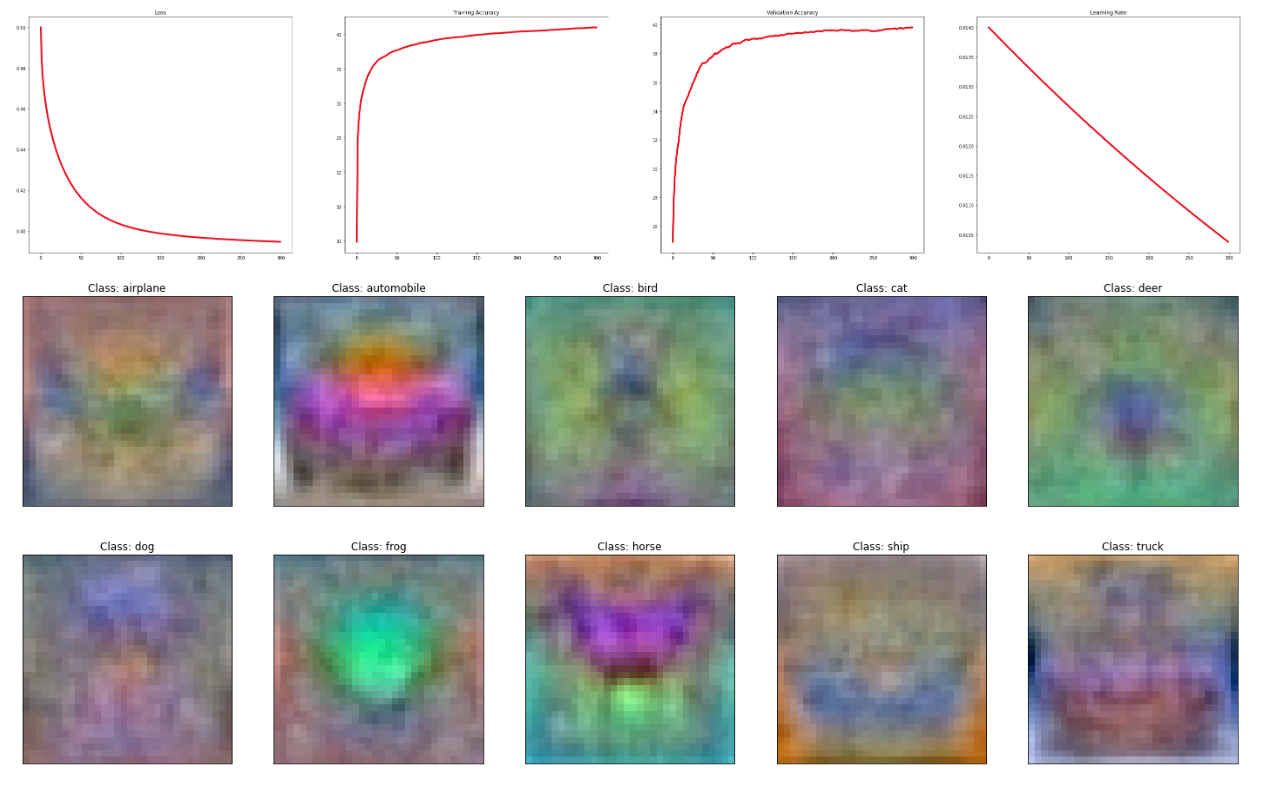
\includegraphics[width=0.9\linewidth]{1_2.PNG}
  \caption{Learning and loss curves with the weights matrix W as 10 images}
  \label{fig:sub1}
\end{subfigure}%
\begin{subfigure}{0.5\textwidth}
  \centering
  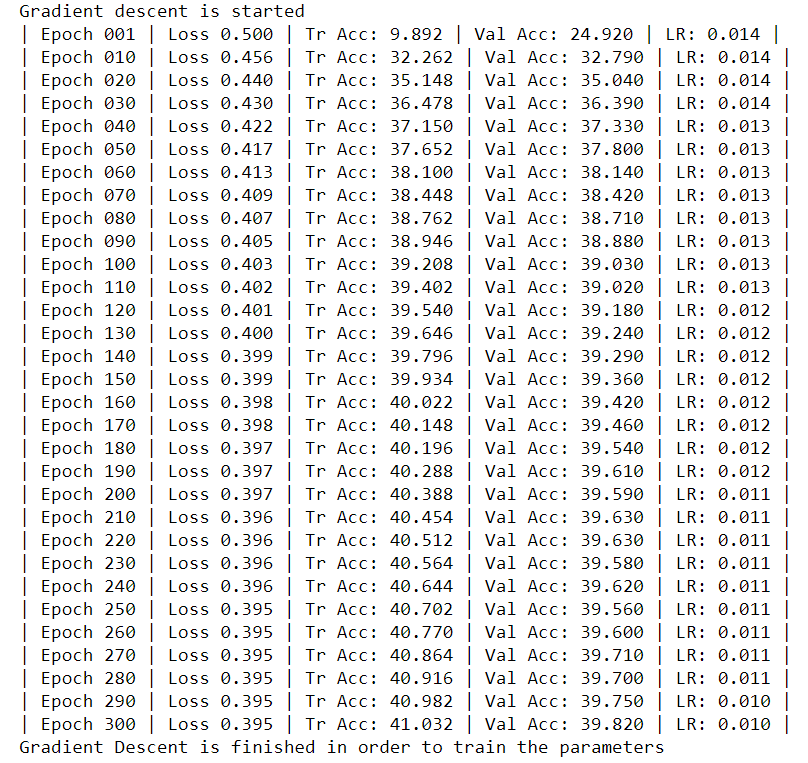
\includegraphics[width=0.7\linewidth]{1_1.PNG}
  \caption{Numerical values of the losses and accuracies (training and validation) with learning rate}
  \label{fig:sub2}
\end{subfigure}
\caption{Acquired results through the implemented linear classifier}
\label{fig:test}
\end{figure}
\end{enumerate}

\paragraph*{Problem 2}
Code a two-layer fully connected network with $H = 200$ hidden nodes. Choose the sigmoid function as the activation function for the hidden nodes. The output layer has no activation function.
\begin{enumerate}[label=(\alph*)]
\item Implement gradient descent and run for 300 epochs.
\newline When we analyse the layer-wise organization of neural network architectures, it is critical to identify that the neural networks are acyclic (in order to avoid infinite loops in the forward pass of a network) and the the outputs of some neurons in a layer become inputs to other neurons in a different layer. In the scenario of fully-connected networks, the neurons between two adjacent layers are fully pairwise connected, but neurons within a single layer share no connections \cite{web1}.

In the python implementation, the same pre-processing steps have been executed except having a normalization since it is necessary to have significant differences in the consecutive weight matrices in order for the model to learn. The hidden layer is of size $DXH = 3072X200$ since there exists 200 hidden nodes as per the requirement. Correspondingly, the bias vector has the size of $200X1$ and further, the activation of the hidden nodes is chosen to be \textit{sigmoid function}. 

Sigmoid is a non-linear function with the mathematical form of \cite{web1},
\begin{equation}
    \sigma (x) = \frac{1}{1+\exp{(-x)}}
\end{equation}
Here, the function takes a real-valued number from the image and “squashes” it into range between 0 and 1 such that large negative numbers become 0 and large positive numbers become 1. The output from this hidden layer (with sigmoid activation) is fed into the last (output) layer (with the weight matrix of the size $200X10$ and the bias vector of the size $10X1$) to acquire the predicted output from the full model. The similar reduction of computational complexity as in Problem 1 is implemented here by re-arranging the train-test samples and the weight-bias matrices. The initial learning rate is chosen to be $1.4X10^{-2}$. 

In the iterations, the forward propagation is executed via the sigmoid activation of the hidden layer (to which the input layer feeds) and then, the acquired matrix from this layer is re-arranged and fed into the last layer to obtain the prediction. The loss is calculated using the simplest method of loss calculation: the mean sum of squared errors function. In order to minimize the total error of the network, the back propagation is implemented using the partial derivations of the loss functions in order to update the weights in each layer. Here, the chain rule for the differentiation is implemented,
\begin{equation}
    \frac{dl}{dw2} = \frac{dl}{dpredict} X \frac{dpredict}{dw2}
\end{equation}

\begin{equation}
    \frac{dl}{dw1} = (\frac{dl}{dpredict}X\frac{dpredict}{dh})X(\frac{dh}{dw1x}X\frac{dw1x}{dw1})
\end{equation}

Afterwards, the weights are adjusted necessarily and training and validation accuracies and losses are calculated and reported similarly to the Problem 1. Finally, the learning rate is decayed.

\item Report the (initial) learning rate, training and testing loss and accuracies.
\newline The following graphs convey the necessary weights matrix using 10 class images (Figure 2(a)) along with the initial learning rate, training and testing accuracies and losses (Figure 2(b)). This two-layer fully connected network outperforms the linear classifier in Problem 1 in terms of training and validation accuracies and the losses within the 300 epochs. Howsoever, the learning and loss curves of this model suggest an observable instability in learning (within the chosen leaning and decaying parameters).
\end{enumerate}

\begin{figure}[H]
\centering
\begin{subfigure}{0.5\textwidth}
  \centering
  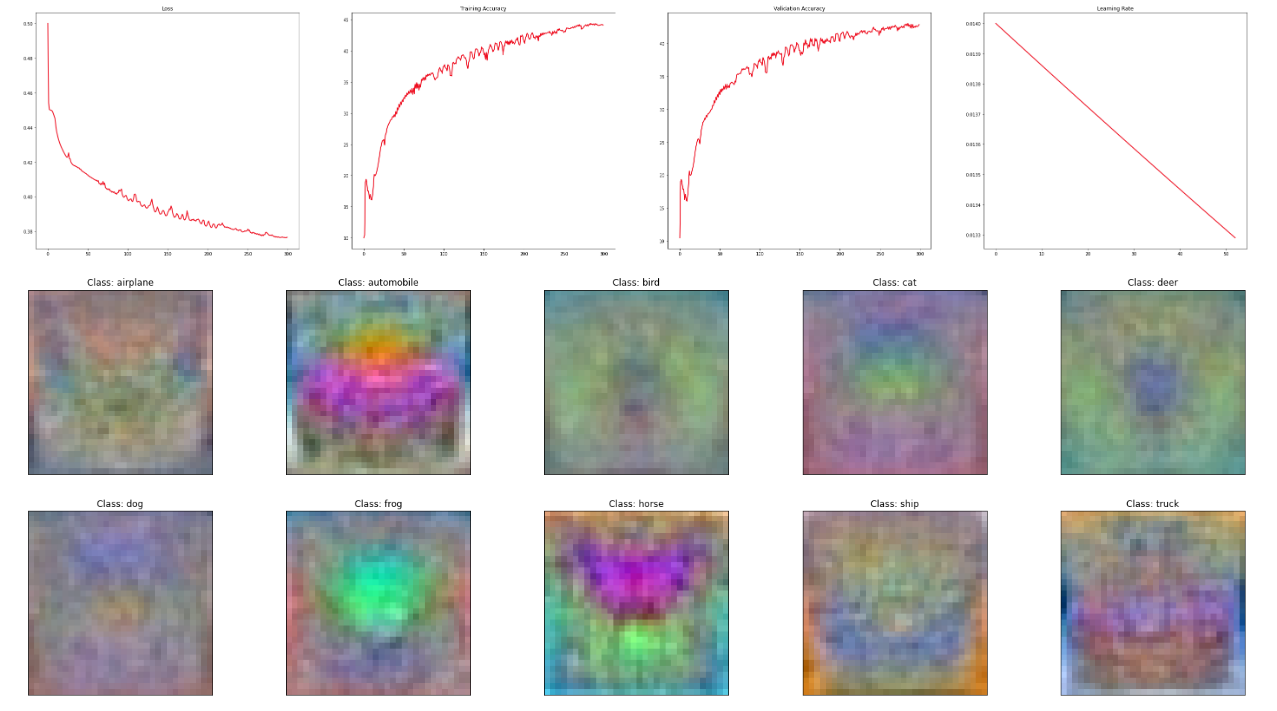
\includegraphics[width=.8\linewidth]{2_2.PNG}
  \caption{Learning and loss curves with the weights matrix W as 10 images}
  \label{fig:sub2}
\end{subfigure}
\begin{subfigure}{0.4\textwidth}
  \centering
  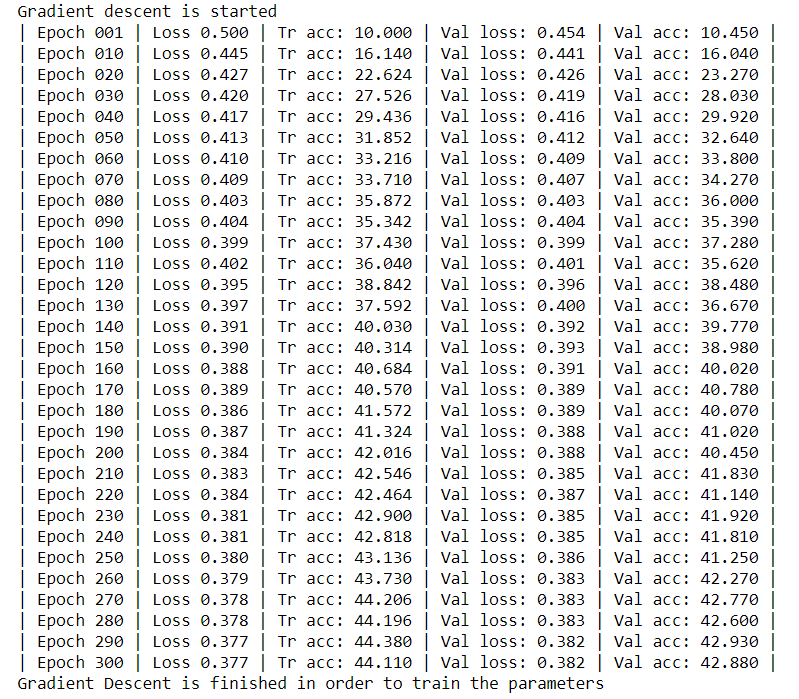
\includegraphics[width=.7\linewidth]{2_1.PNG}
  \caption{Numerical values of the losses and accuracies (training and validation) with learning rate}
  \label{fig:sub2}
\end{subfigure}
\caption{Acquired results through the implemented two-layer fully connected network}
\label{fig:test}
\end{figure}

\paragraph*{Problem 3}
Modify the code in item 2 to carry out stochastic gradient descent with a batch size of 500 (Report training and testing loss and accuracies and Compare results with item 2).

\newline Stochastic gradient descent (SGD) is a form of mini-batch gradient descent where the gradient is calculated using a selected number of batches in the training data rather than computing the full loss function over the entire training set in order to perform only a single parameter update. In implementing stochastic gradient descent in the two-layer fully connected network in the problem 2, a batch size of 500 (which is a hyper-parameter that is commonly hard to cross-validate) is used since it is generally considered that the gradient from a mini-batch is a good approximation of the gradient of the full objective \cite{web1}.

In the python implementation, major changes have been implemented to the code in Problem 2 in the gradient descent to manipulate the required stochastic nature. Here, since the number of samples are 50000 in the dataset and the batch size is 500, then there is a need to execute 100 groups for each epoch in order to update the weights. The required indices are obtained through \textit{numpy random} function from the re-arranged training sample sets. Here, the sigmoid activation in the hidden layer in forward propagation and the necessary backward propagation is limited as per the batch size. The rest of the implementation is quite similar to the Problem 2.   

\begin{figure}[H]
    \centering
    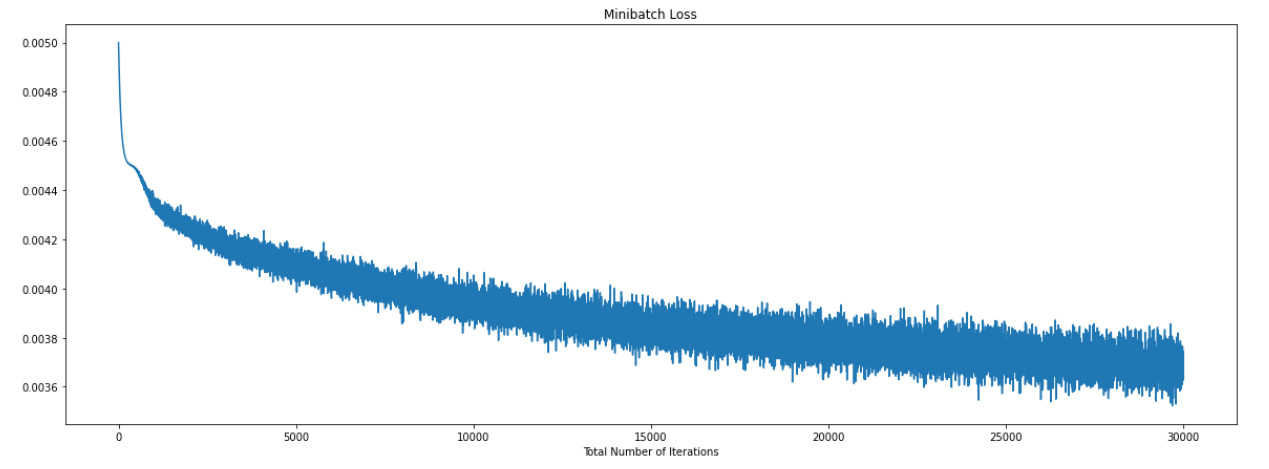
\includegraphics[width=0.6\textwidth]{3_2.PNG}
    \caption{Mini-batch loss vs total number of iterations }
    \label{fig: PaleBlueDot}    
\end{figure}

Afterwards, as in problem (3), the \textit{warpPerspective} is utilized in order to apply the obtained transformation into stitching as per required.

\begin{figure}[H]
\centering
\begin{subfigure}{.5\textwidth}
  \centering
  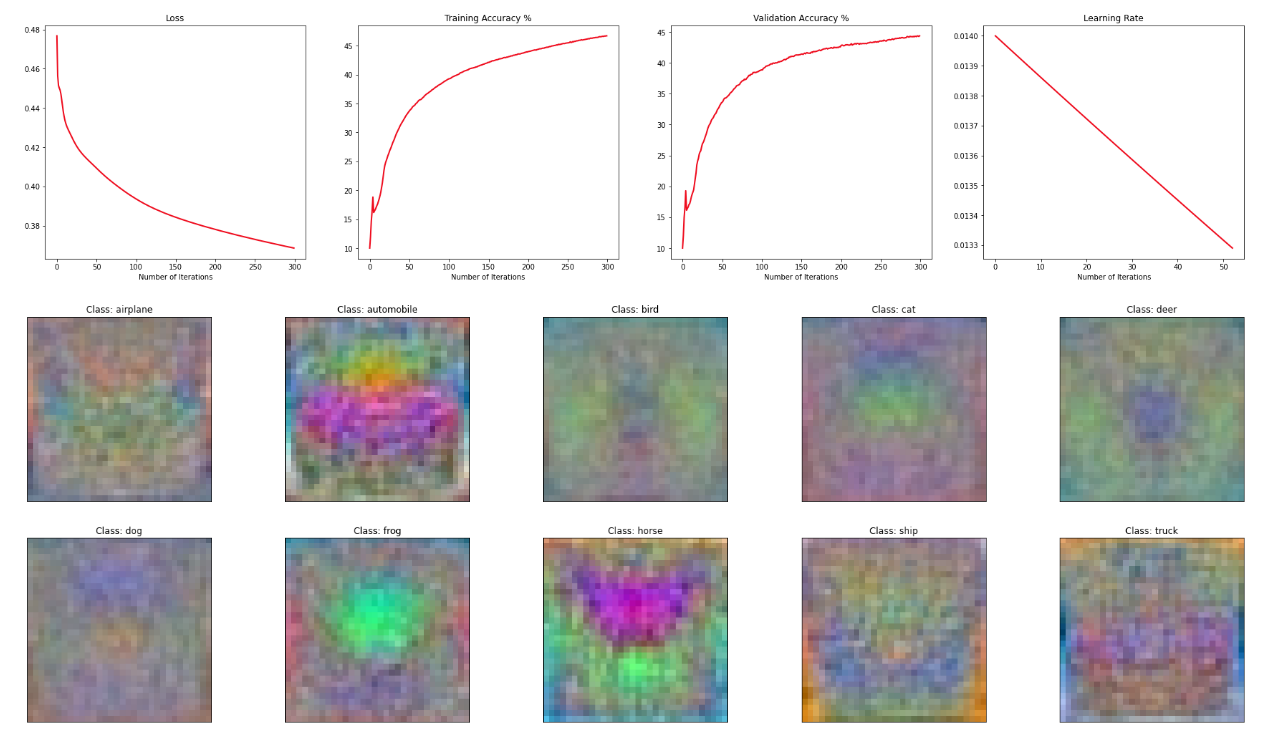
\includegraphics[width=0.9\linewidth]{3_3.PNG}
  \caption{Learning and loss curves with the weights matrix W as 10 images}
  \label{fig:sub1}
\end{subfigure}%
\begin{subfigure}{0.5\textwidth}
  \centering
  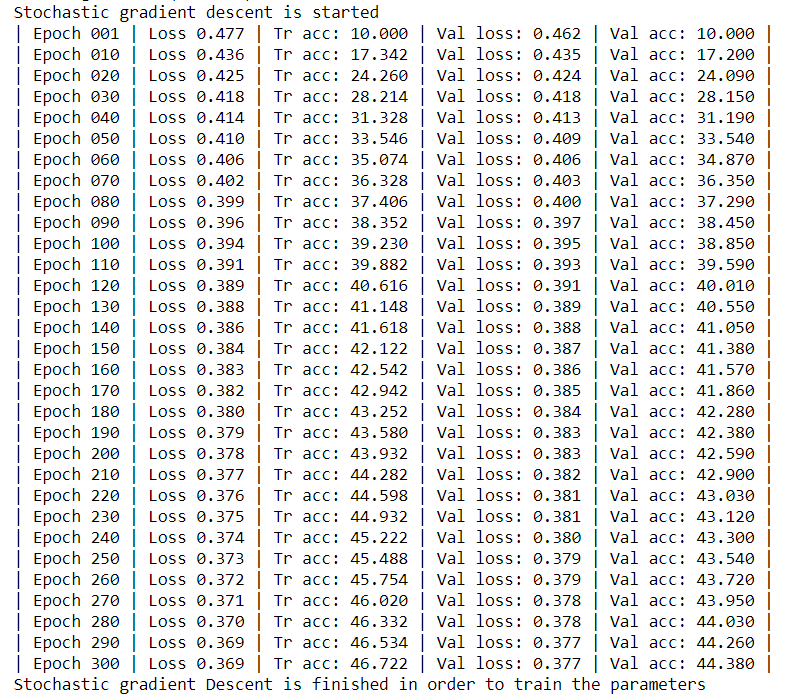
\includegraphics[width=0.6\linewidth]{3_1.PNG}
  \caption{Numerical values of the losses and accuracies (training and validation) with learning rate}
  \label{fig:sub2}
\end{subfigure}
\caption{Acquired results through the implemented random gradient descent}
\label{fig:test}
\end{figure}

The losses and accuracies of the training and validation datasets are comparatively higher in stochastic gradient descent method when compared with the two-layer fully connected layer in Problem 2 within the given number of epochs. Further, the latter method in Problem 3 shows a stable learning potential than the method in Problem 2. Even though, it is expected to have a much faster convergence (by using SDG) by evaluating the mini-batch gradients to perform more frequent parameter update, the practise shows a higher time consumption in SDG than the previous method. This may be due to vectorized code optimizations in the previous method can be computationally much more efficient to evaluate the gradient for 100 examples, than the gradient for one example 100 times. Thus, reduce the efficiency of SGD. 

\paragraph*{Problem 4}
Construct a CNN using \textit{Keras.models.Sequential} (with the following configuration: C32, C64, C64, F64, F10. All three convolutions layers are 3x3. Max pooling (2x2) follows each convolution layer. Use SDG (with momentum) with a batch size of 50 and \textit{CategoricalCrossentropy} as the loss (Include how many learnable parameters are there in this network?, report the parameters such as the learning rate and momentum and Report training and testing loss and accuracies)

Here, the implementation is a sequential CNN model from keras deep learning framework which has the configuration of C32, C64, C64, F64, F10. Since CNNs are made up of neurons that have learnable weights and biases, this developed framework has 73418 learnable parameters as the model summary states. In each $3X3$ convolution layer (which is computing the output of neurons that are connected to local regions in the input, each computing a dot product between their weights and a small region they are connected to in the input volume \cite{web1}), the \textit{relu} elementwise activation has been implemented which has the mathematical expression of $f(x)=\max(0,x)$. Following each convolutional layer, there is a max pooling layer of size $2X2$ to perform a down-sampling operation along the spatial dimensions (width, height). At the final stage of the architecture, there are two dense layers each has 64 outputs and 10 outputs respectively which are computing the class scores. Here, it is required to implement the stochastic gradient descent as the keras optimizing method with the momentum (0.9) as chosen. Further, the loss function of categorical cross-entropy which in simple form has the $loss=-\sum_{i=1}^{outputSize} y_iX\log{\hat{y_i}}$.  

\begin{figure}[H]
\centering
\begin{subfigure}{0.4\textwidth}
  \centering
  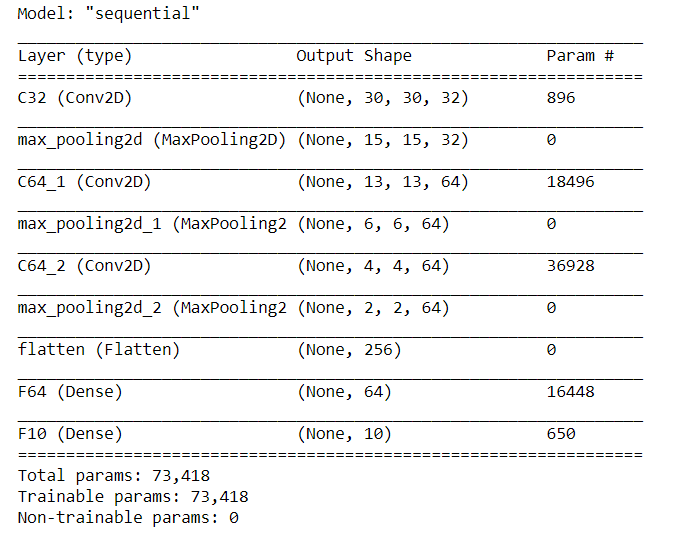
\includegraphics[width=.9\linewidth]{4_1.PNG}
  \caption{Sequential model summary}
  \label{fig:sub2}
\end{subfigure}
\begin{subfigure}{0.4\textwidth}
  \centering
  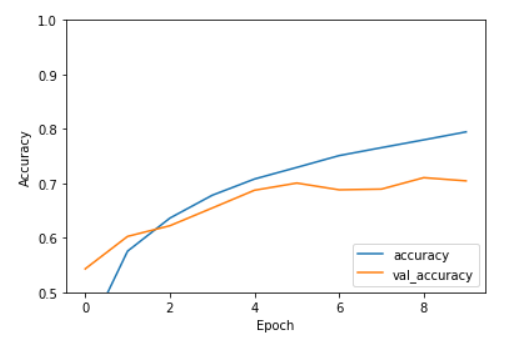
\includegraphics[width=.9\linewidth]{4_2.PNG}
  \caption{Training and validation learning plots}
  \label{fig:sub2}
\end{subfigure}
\caption{Acquired results through the implemented convolutional neural network}
\label{fig:test}
\end{figure}



\bibliography{references}

\end{document}

